\begin{figure}[h]
    \centering
    \begin{subfigure}[b]{0.48\textwidth}
        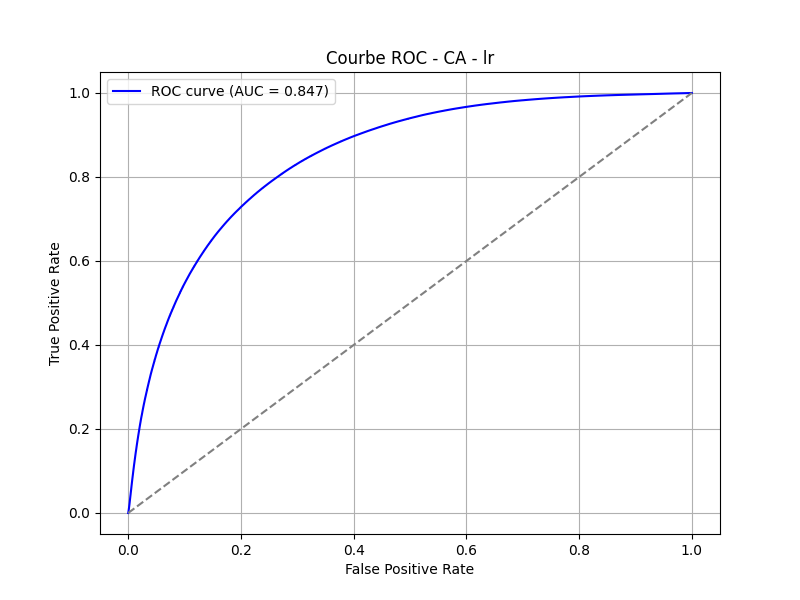
\includegraphics[width=\textwidth]{Images/curve_roc_folktables/roc_curve_CA_lr.png}
        \caption{Curve ROC (AUC = 0.847): model = Logistic Regression}
        \label{fig:ca_lr}
    \end{subfigure}
    \hfill
    \begin{subfigure}[b]{0.48\textwidth}
        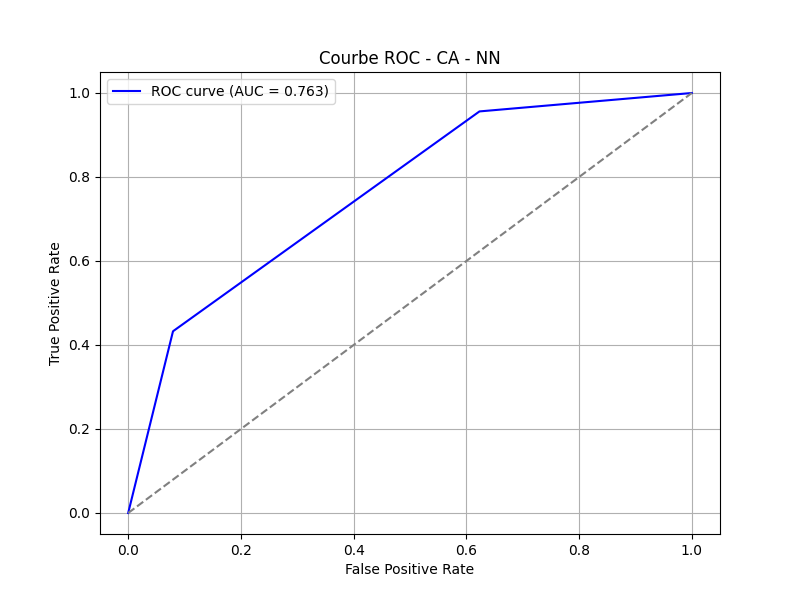
\includegraphics[width=\textwidth]{Images/curve_roc_folktables/roc_curve_CA_NN.png}
        \caption{Curve ROC (AUC = 0.763): model = Neural Network}
        \label{fig:ca_nn}
    \end{subfigure}

    \begin{subfigure}[b]{0.48\textwidth}
        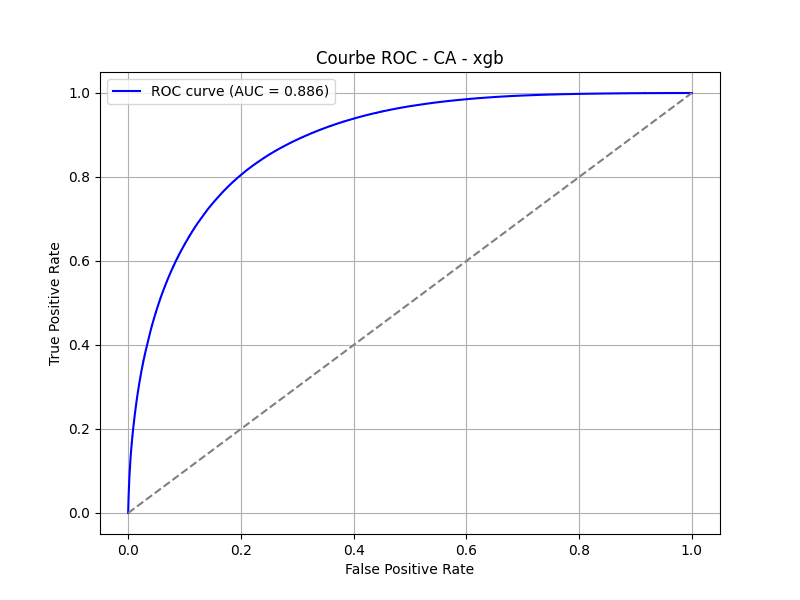
\includegraphics[width=\textwidth]{Images/curve_roc_folktables/roc_curve_CA_xgb.png}
        \caption{Curve ROC (AUC = 0.886): model = XGBoost}
        \label{fig:ca_xgb}
    \end{subfigure}
    \hfill
    \begin{subfigure}[b]{0.48\textwidth}
        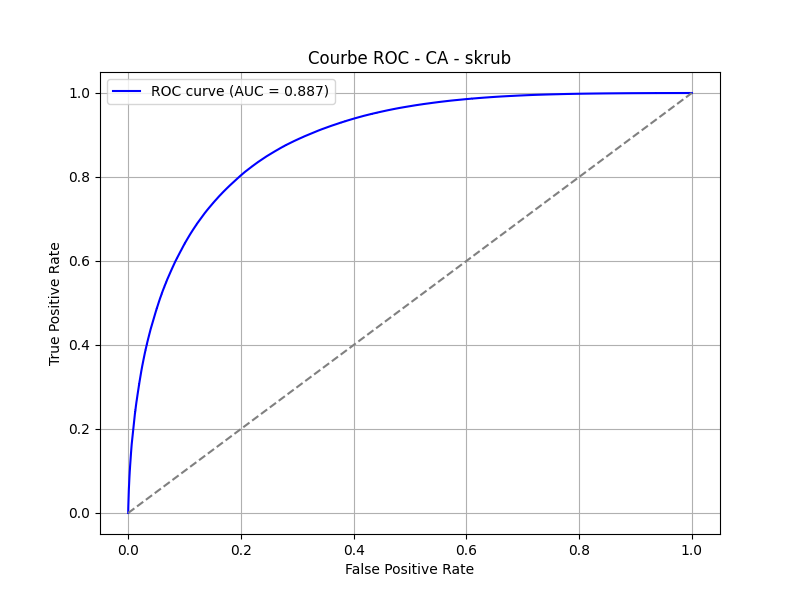
\includegraphics[width=\textwidth]{Images/curve_roc_folktables/roc_curve_CA_skrub.png}
        \caption{Curve ROC (AUC = 0.887): model = HistGradientBoosting}
        \label{fig:ca_skrub}
    \end{subfigure}
    \caption{Comparison of the models trained on the sub dataset of the California state}
    \label{fig:roc_ca}
\end{figure}

\begin{figure}[h]
    \centering
    \begin{subfigure}[b]{0.48\textwidth}
        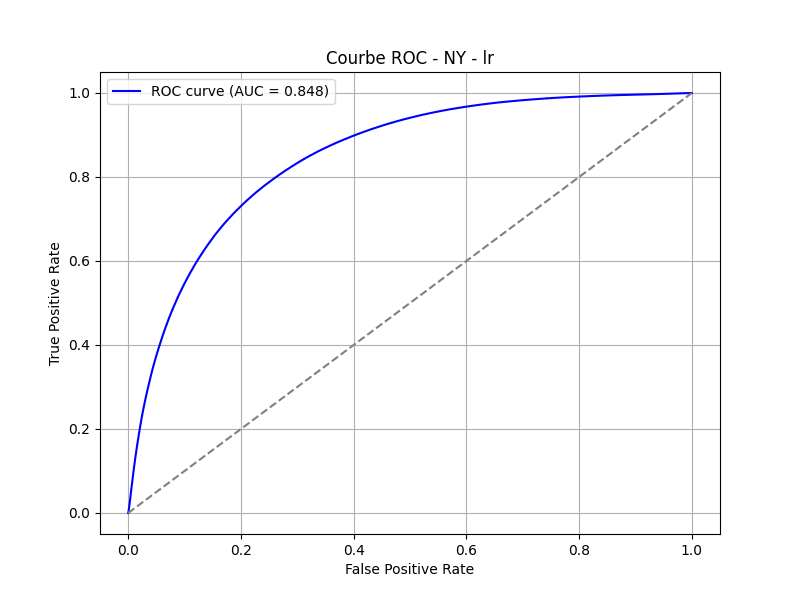
\includegraphics[width=\textwidth]{Images/curve_roc_folktables/roc_curve_NY_lr.png}
        \caption{Curve ROC (AUC = 0.848): model = Logistic Regression}
        \label{fig:NY_lr}
    \end{subfigure}
    \hfill
    \begin{subfigure}[b]{0.48\textwidth}
        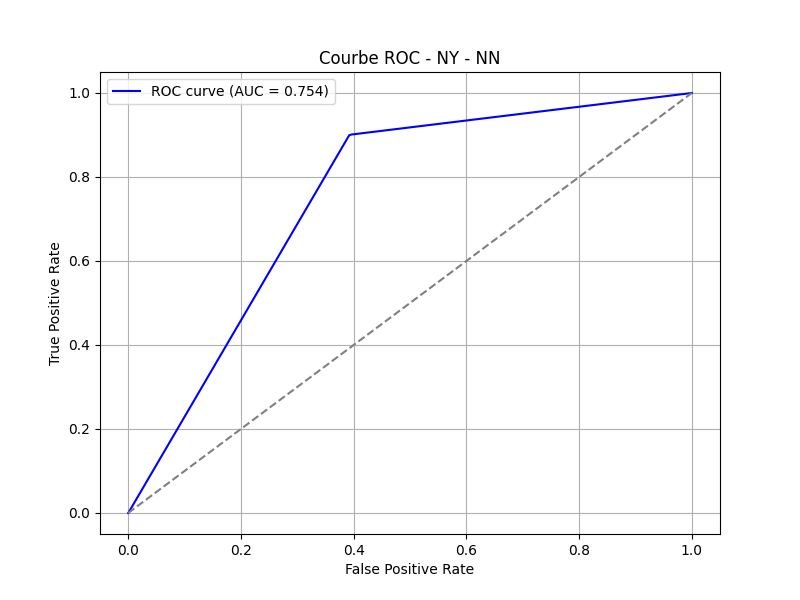
\includegraphics[width=\textwidth]{Images/curve_roc_folktables/roc_curve_NY_NN.png}
        \caption{Curve ROC (AUC = 0.754): model = Neural Network}
        \label{fig:NY_nn}
    \end{subfigure}

    \begin{subfigure}[b]{0.48\textwidth}
        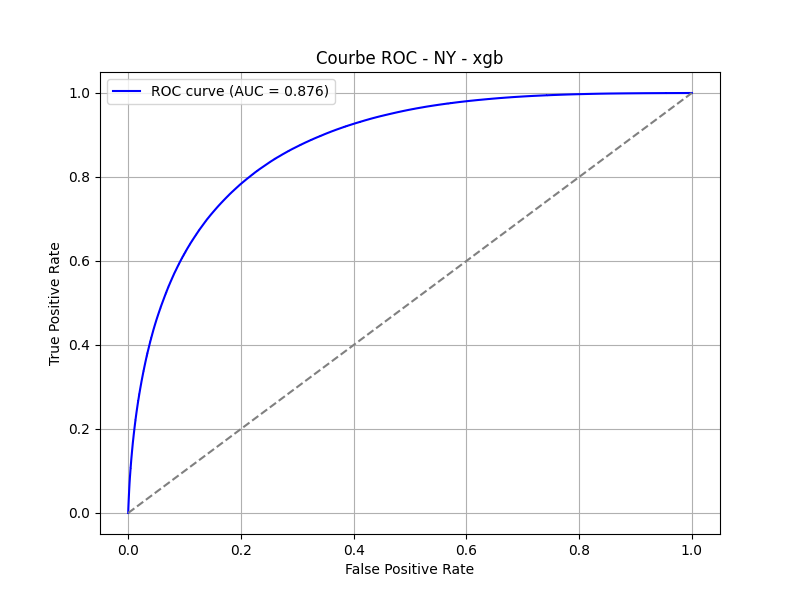
\includegraphics[width=\textwidth]{Images/curve_roc_folktables/roc_curve_NY_xgb.png}
        \caption{Curve ROC (AUC = 0.876): model = XGBoost}
        \label{fig:NY_xgb}
    \end{subfigure}
    \hfill
    \begin{subfigure}[b]{0.48\textwidth}
        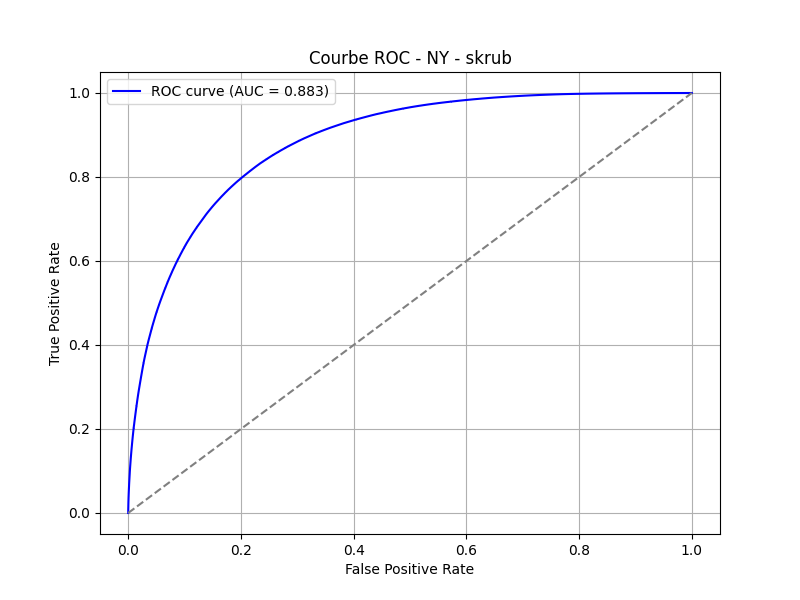
\includegraphics[width=\textwidth]{Images/curve_roc_folktables/roc_curve_NY_skrub.png}
        \caption{Curve ROC (AUC = 0.883): model = HistGradientBoosting}
        \label{fig:NY_skrub}
    \end{subfigure}
    \caption{Comparison of the models trained on the sub dataset of the New York state}
    \label{fig:roc_ny}
\end{figure}